\documentclass[a4paper, 14pt]{extarticle}

% Поля
%--------------------------------------
\usepackage{geometry}
\geometry{a4paper,tmargin=2cm,bmargin=2cm,lmargin=3cm,rmargin=1cm}
%--------------------------------------


%Russian-specific packages
%--------------------------------------
\usepackage[T2A]{fontenc}
\usepackage[utf8]{inputenc} 
\usepackage[english, main=russian]{babel}
%--------------------------------------

\usepackage{textcomp}

% Красная строка
%--------------------------------------
\usepackage{indentfirst}               
%--------------------------------------             


%Graphics
%--------------------------------------
\usepackage{graphicx}
\graphicspath{ {./images/} }
\usepackage{wrapfig}
%--------------------------------------

% Полуторный интервал
%--------------------------------------
\linespread{1.3}                    
%--------------------------------------

%Выравнивание и переносы
%--------------------------------------
% Избавляемся от переполнений
\sloppy
% Запрещаем разрыв страницы после первой строки абзаца
\clubpenalty=10000
% Запрещаем разрыв страницы после последней строки абзаца
\widowpenalty=10000
%--------------------------------------

%Списки
\usepackage{enumitem}

%Подписи
\usepackage{caption} 

%Гиперссылки
\usepackage{hyperref}

\hypersetup {
	unicode=true
}

%Рисунки
%--------------------------------------
\DeclareCaptionLabelSeparator*{emdash}{~--- }
\captionsetup[figure]{labelsep=emdash,font=onehalfspacing,position=bottom}
%--------------------------------------

\usepackage{tempora}

%Листинги
%--------------------------------------
\usepackage{listings}
\lstset{
  basicstyle=\ttfamily\footnotesize, 
  %basicstyle=\footnotesize\AnkaCoder,        % the size of the fonts that are used for the code
  breakatwhitespace=false,         % sets if automatic breaks shoulbd only happen at whitespace
  breaklines=true,                 % sets automatic line breaking
  captionpos=t,                    % sets the caption-position to bottom
  inputencoding=utf8,
  frame=single,                    % adds a frame around the code
  keepspaces=true,                 % keeps spaces in text, useful for keeping indentation of code (possibly needs columns=flexible)
  keywordstyle=\bf,       % keyword style
  numbers=left,                    % where to put the line-numbers; possible values are (none, left, right)
  numbersep=5pt,                   % how far the line-numbers are from the code
  xleftmargin=25pt,
  xrightmargin=25pt,
  showspaces=false,                % show spaces everywhere adding particular underscores; it overrides 'showstringspaces'
  showstringspaces=false,          % underline spaces within strings only
  showtabs=false,                  % show tabs within strings adding particular underscores
  stepnumber=1,                    % the step between two line-numbers. If it's 1, each line will be numbered
  tabsize=2,                       % sets default tabsize to 8 spaces
  title=\lstname                   % show the filename of files included with \lstinputlisting; also try caption instead of title
}
%--------------------------------------

%%% Математические пакеты %%%
%--------------------------------------
\usepackage{amsthm,amsfonts,amsmath,amssymb,amscd}  % Математические дополнения от AMS
\usepackage{mathtools}                              % Добавляет окружение multlined
\usepackage[perpage]{footmisc}
%--------------------------------------

%--------------------------------------
%			НАЧАЛО ДОКУМЕНТА
%--------------------------------------

\begin{document}

%--------------------------------------
%			ТИТУЛЬНЫЙ ЛИСТ
%--------------------------------------
\begin{titlepage}
\thispagestyle{empty}
\newpage


%Шапка титульного листа
%--------------------------------------
\vspace*{-60pt}
\hspace{-65pt}
\begin{minipage}{0.3\textwidth}
\hspace*{-20pt}\centering

\includegraphics[width=\textwidth]{emblem}
\end{minipage}
\begin{minipage}{0.67\textwidth}\small \textbf{
\vspace*{-0.7ex}
\hspace*{-6pt}\centerline{Министерство науки и высшего образования Российской Федерации}
\vspace*{-0.7ex}
\centerline{Федеральное государственное бюджетное образовательное учреждение }
\vspace*{-0.7ex}
\centerline{высшего образования}
\vspace*{-0.7ex}
\centerline{<<Московский государственный технический университет}
\vspace*{-0.7ex}
\centerline{имени Н.Э. Баумана}
\vspace*{-0.7ex}
\centerline{(национальный исследовательский университет)>>}
\vspace*{-0.7ex}
\centerline{(МГТУ им. Н.Э. Баумана)}}
\end{minipage}
%--------------------------------------

%Полосы
%--------------------------------------
\vspace{-25pt}
\hspace{-35pt}\rule{\textwidth}{2.3pt}

\vspace*{-20.3pt}
\hspace{-35pt}\rule{\textwidth}{0.4pt}
%--------------------------------------

\vspace{1.5ex}
\hspace{-35pt} \noindent \small ФАКУЛЬТЕТ\hspace{80pt} <<Информатика и системы управления>>

\vspace*{-16pt}
\hspace{47pt}\rule{0.83\textwidth}{0.4pt}

\vspace{0.5ex}
\hspace{-35pt} \noindent \small КАФЕДРА\hspace{50pt} <<Теоретическая информатика и компьютерные технологии>>

\vspace*{-16pt}
\hspace{30pt}\rule{0.866\textwidth}{0.4pt}
  
\vspace{11em}

\begin{center}
\Large {\bf Лабораторная работа № 1} \\
\large {\bf по курсу <<Численные методы линейной алгебры>>} \\
\large <<Подготовка вспомогательных средств разработки>>
\end{center}\normalsize

\vspace{8em}


\begin{flushright}
  {Студентка группы ИУ9-72Б Самохвалова П. С. \hspace*{15pt}\\
  \vspace{2ex}
  Преподаватель Посевин Д. П.\hspace*{15pt}}
\end{flushright}

\bigskip

\vfill
 

\begin{center}
\textsl{Москва 2023}
\end{center}
\end{titlepage}
%--------------------------------------
%		КОНЕЦ ТИТУЛЬНОГО ЛИСТА
%--------------------------------------

\renewcommand{\ttdefault}{pcr}

\setlength{\tabcolsep}{3pt}
\newpage
\setcounter{page}{2}

\section{Цель работы}\label{Sect::goal}

Подготовить методы необходимые для решения задач численных методов
линейной алгебры.

\section{Задание}\label{Sect::task}

\begin{enumerate}
    \item Подготовить методы для выполнения операций с векторами: вычисление скалярного произведения двух векторов, вычисление Евклидовой нормы вектора.
    \item Подготовить методы для выполнения операций с матрицами: умножение матрицы на матрицу, умножение матрицы на вектор, транспонирование матрицы.
    \item Подготовить метод построения графика произвольной функции от одной переменной.
    \item Реализовать оценку погрешности вычисления объема шара зажатого цилиндром тремя способами при двух различных приближениях вычисления значения $2^{0.5}$: 7/5 и 17/12.
\end{enumerate}

\section{Практическая реализация}\label{Sect::code}

Исходный код программы представлен в листингах~\ref{lst:code1}--~\ref{lst:code2}.

\begin{lstlisting}[language={python},caption={Методы для выполнения операций с матрицами и векторами},label={lst:code1}]
from matplotlib import pyplot as plt


def scalar_mult_vec(vec1, vec2):
    n = len(vec1)
    s = 0
    for i in range(n):
        s += vec1[i] * vec2[i]
    return s


def norm_vec(vec):
    n = len(vec)
    s = 0
    for i in range(n):
        s += vec[i] ** 2
    norm = s ** 0.5
    return norm


def mult_matr_matr(matr1, matr2):
    n1 = len(matr1)
    m1 = len(matr1[0])
    m2 = len(matr2[0])
    matr = [[0] * m2 for i in range(n1)]
    for i in range(n1):
        for j in range(m2):
            for k in range(m1):
                matr[i][j] += matr1[i][k] * matr2[k][j]
    return matr


def mult_matr_vec(matr, vec):
    n = len(vec)
    m = len(matr[0])
    vec1 = [0] * n
    for i in range(n):
        for j in range(m):
            vec1[i] += matr[i][j] * vec[j]
    return vec1


def transp_matr(matr):
    n = len(matr)
    m = len(matr[0])
    matr1 = [[0] * n for i in range(m)]
    for i in range(m):
        for j in range(n):
            matr1[i][j] = matr[j][i]
    return matr1


def plot_func(func, x):

    y = [func(x[i]) for i in range(len(x))]

    plt.xlabel('x')
    plt.ylabel('y')
    plt.grid()
    plt.plot(x, y)
    plt.show()

\end{lstlisting}

\begin{lstlisting}[language={python},caption={Оценка погрешностей},label={lst:code2}]
import math

from num_methods import *


def calc_err(x):

    true_value = 0.005051

    v1 = (x - 1) ** 6
    v2 = (3 - 2 * x) ** 3
    v3 = 99 - 70 * x

    print("Relative error at the root of 2, equal to", x)

    print("First method -", abs(true_value - v1) / true_value)
    print("Second method -", abs(true_value - v2) / true_value)
    print("Third method -", abs(true_value - v3) / true_value)
    print()


def calc_err1(x):

    delta_x = abs(math.sqrt(2) - x)

    v1 = 6 / (math.sqrt(2) - 1)
    v2 = 6 / (3 - 2 * math.sqrt(2))
    v3 = 70 / (99 - 70 * math.sqrt(2))

    print("Error estimation with a root of 2, equal to", x)

    print("First method -", v1 * delta_x)
    print("Second method -", v2 * delta_x)
    print("Third method -", v3 * delta_x)
    print()


print(scalar_mult_vec([1, 2, 3], [4, 5, 6]))
print(norm_vec([1, 2, 3]))
print()

print(mult_matr_matr([[1, 2], [3, 4], [5, 6]], [[1, 2, 3, 4, 5],
                                                [6, 7, 8, 9, 10]]))
print(mult_matr_vec([[1, 2, 3], [4, 5, 6], [7, 8, 9]], [1, 2, 3]))
print(transp_matr([[1, 2], [3, 4], [5, 6]]))
print()

plot_func(lambda x: x ** 2, [1, 2, 3, 4, 5])

calc_err(7 / 5)
calc_err(17 / 12)

calc_err1(7 / 5)
calc_err1(17 / 12)

\end{lstlisting}

\section{Результаты}\label{Sect::res}

Результаты работы программы представлены на рисунках~\ref{fig:img1}~--~\ref{fig:img3}.

\begin{figure}[!htb]
	\centering
	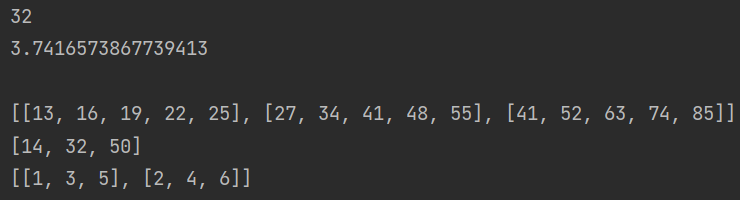
\includegraphics[width=0.8\textwidth]{img1}
\caption{Результаты работы операций с матрицами и векторами}
\label{fig:img1}
\end{figure}

\begin{figure}[!htb]
	\centering
	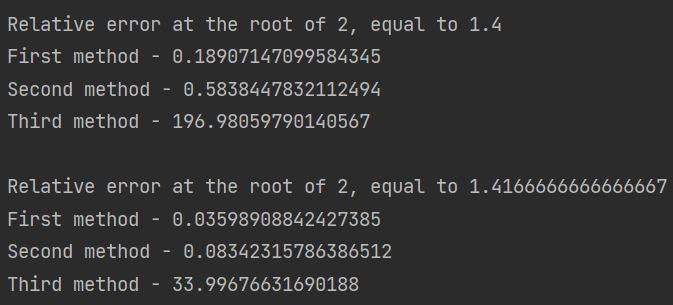
\includegraphics[width=0.8\textwidth]{img2}
\caption{Относительные погрешности}
\label{fig:img2}
\end{figure}

\begin{figure}[!htb]
	\centering
	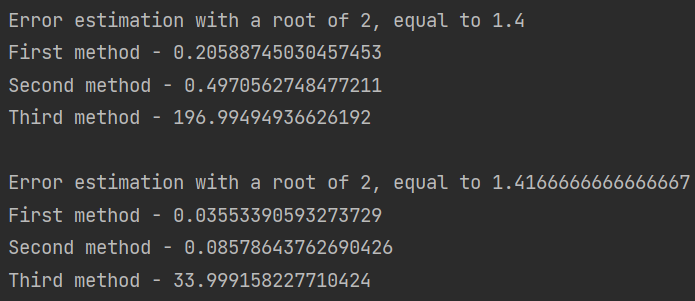
\includegraphics[width=0.8\textwidth]{img3}
\caption{Оценка погрешностей}
\label{fig:img3}
\end{figure}

\section{Выводы}\label{Sect::conclusion}

В результате выполнения лабораторной работы были реализованы методы для выполнения операций с матрицами и векторами, был реализован метод построения графика произвольной функции от одной переменной, была реализована оценка погрешности вычисления объема шара зажатого цилиндром тремя способами при двух различных приближениях вычисления значения $2^{0.5}$: 7/5 и 17/12.

\end{document}
